\documentclass[12pt]{standalone}

% main document, called main.tex \usepackage{tikz}
% \usetikzlibrary{external}
% \tikzexternalize % activate!

\usepackage{tikz}

\usetikzlibrary{decorations.markings}
\usetikzlibrary{math}
\usetikzlibrary{fadings}



\begin{document}
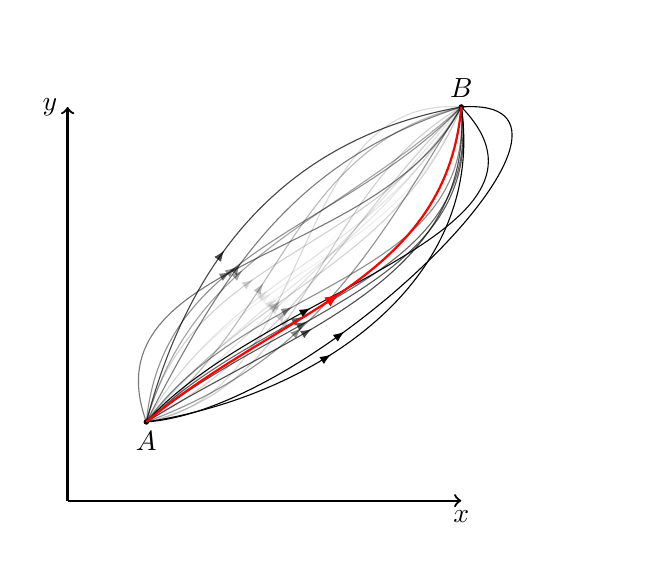
\begin{tikzpicture}

\tikzmath{
    \inTheta={51.81624114,   -3.22471934,   44.52663386,   12.79477274,
         70.68496187,   34.98091436,   20.09273327,   27.35130173,
         61.14789197,   47.39290738,   30.79834894,    2.46229032,
         76.37915647,   49.55898955,  103.65893003,  -65.38835544,
         -6.18288859,   65.77022135,  110.12138352,   -7.14611594,
         83.00933352,  -11.52450939,   27.67690678,   32.33649643,
          3.79456554};
    \outTheta={ 279.10006082,  268.74437783,  216.56477818,  242.92657086,
        183.46275938,  203.14523784,  314.72883253,  184.6162975 ,
        192.8076593 ,  298.22349721,  222.84202208,  265.36860045,
        290.44239534,  166.45589606,  215.68427653,  268.98069034,
        215.71141227,  245.06678041,  250.62213771,  257.63982239,
        285.39220064,  155.77481395,  234.84268398,  232.70925945,
        229.22827614};
    \Strength={0.30630376,  0.59577422,  0.05157676,  0.32475292,  0.43546426,
        0.07667131,  0.74261066,  0.14727696,  0.31314719,  0.45883933,
        0.07801871,  0.53706564,  0.22066107,  0.40878074,  0.44033863,
        1.        ,  0.27139055,  0.00455688,  0.25587543,  0.54924184,
        0.14499582,  0.08227476,  0.17597943,  0.13197441,  0.29431879};
}

\draw[white] (6.0, 6.0) rectangle (-0.5,-0.5);

% Coordinates
\coordinate (Start) at (1,1);
\coordinate (Stop) at (5,5);

% Draws x-axis
\draw [->,thick] (0,0) --  (5, 0) node [below] {$x$};
\fill (Start) circle (1pt) node [below] {$A$};
% Draws y-axis
\draw [->,thick] (0,0) --  (0, 5) node [left] {$y$};
\fill (Stop) circle (1pt) node [above] {$B$};

% Marks points
\foreach \x/\y/\str in {
{75.3187/190.0408/0.7286},
{39.7967/230.4210/0.1186},
{12.9218/210.2534/0.1935},
{49.2664/237.9966/0.0974},
{48.1915/314.1537/0.9595},
{62.8694/197.6769/0.5044},
{44.1743/277.3271/0.5933},
{32.0323/274.0566/0.6923},
{39.5288/278.2094/0.6550},
{9.5157/176.0789/0.1500},
{28.9922/225.0038/0.1787},
{84.3960/225.8472/0.4303},
{-1.0324/179.8976/0.0104},
{59.9838/239.9771/0.1},
{109.9675/242.5455/0.5293},
{61.0783/247.1942/0.0683},
{20.4381/238.6206/0.4262},
{51.3961/247.2784/0.1773},
{43.3658/225.8432/0.0277},
{74.0469/221.8953/0.3589},
{74.8679/238.6053/0.1815},
{38.2038/193.6668/0.2739},
{54.1859/274.2840/0.4476},
{8.6877/278.2777/1.0000},
{79.5065/252.6087/0.0770}
} {
    \path [
        draw,
        decoration={markings, mark=at position 0.4 with {\arrow[black]{latex}}}, 
        postaction={decorate},
        opacity=\str,
        ] 
        (Start) to[out=\x, in=\y] (Stop);
}


% Draws lines
\path[
    draw,
    red,
    thick,
    decoration={markings, mark=at position 0.5 with {\arrow[red]{latex}}},
    postaction={decorate},
    ]
    (Start) to[out=40, in=265] (Stop);


% % Inner path
% \path[
%     draw,
%     thick,
%     decoration={markings, mark=at position 0.625 with {\arrow[black]{latex}}},
%     postaction={decorate}
%     ]
%     (C) arc (100:440:1.2) to[out=170, in=10] (A);

\end{tikzpicture}
\end{document}